\documentclass[11pt]{article}
\usepackage[margin=1in]{geometry}
\usepackage{graphicx}
\usepackage{float}
\usepackage[hidelinks]{hyperref}
\usepackage{enumitem}
\setlist{nosep,leftmargin=*,labelsep=0.5em}

\title{DSS Application Design Document}
\author{Group 198}
\date{\today}

\begin{document}
\maketitle
\tableofcontents
\newpage

\section{Overview}
TBD.

\section{Milestone Design Document (50\%)}
\subsection{Application Overview}
TBD.

\subsection{Message Formats for Implemented Commands}
This milestone uses a common message envelope for all requests and responses. Individual commands define their own bodies and semantics.

\subsubsection{Envelope Format (Common to All Messages)}
\paragraph{Envelope}
\begin{verbatim}
{
  "version": 1,
  "message_id": "<role>-<pid>-<timestamp_ms>-<counter>",
  "message_type": "<command_or_response>",
  "status_code": "SUCCESS | FAILURE (optional on requests)",
  "reason": "Optional explanation on FAILURE",
  "body": { /* command-specific fields */ }
}
\end{verbatim}

\noindent\textbf{Message ID Format}\par
\noindent\textbf{Pattern:} \texttt{<role>-<pid>-<timestamp\_ms>-<counter>} (e.g., \texttt{user1-4123-1732665001123-00042}).\par
\begin{tabular}{@{}ll@{}}
\textbf{Role}: & user name or disk name (e.g., \texttt{manager}, \texttt{user1}, \texttt{diskA}) \\
\textbf{PID}: & process ID of the sender \\
\textbf{Timestamp}: & current time in milliseconds \\
\textbf{Counter}: & incremented each time this process sends a message \\
\end{tabular}

\noindent\textbf{Purpose:} match requests and responses, enable retries on UDP, deduplicate requests, and simplify logging.

\subsubsection{Command: \texttt{register\_user}}
\noindent\textbf{Purpose}\par
\medskip
\noindent Register a user process with the manager.
\paragraph{Request}
\begin{verbatim}
{
  "version": 1,
  "message_id": "user1-4123-1732665001123-00001",
  "message_type": "register_user",
  "body": {
    "user_name": "User1",
    "ipv4_address": "192.0.2.10",
    "management_port": 2101,
    "command_port": 2102
  }
}
\end{verbatim}
\paragraph{Response}
\begin{verbatim}
{
  "version": 1,
  "message_id": "user1-4123-1732665001123-00001",
  "message_type": "register_user_response",
  "status_code": "SUCCESS",
  "reason": null
}
\end{verbatim}
On failure: \texttt{status\_code: "FAILURE"} with a \texttt{reason}. Manager ensures unique user name and ports.

\subsubsection{Command: \texttt{register\_disk}}
\noindent\textbf{Purpose}\par
\medskip
\noindent Register a disk process with the manager.
\paragraph{Request}
\begin{verbatim}
{
  "version": 1,
  "message_id": "diskA-6123-1732665001567-00001",
  "message_type": "register_disk",
  "body": {
    "disk_name": "DiskA",
    "ipv4_address": "192.0.2.11",
    "management_port": 2201,
    "command_port": 2202
  }
}
\end{verbatim}
\paragraph{Response}
\begin{verbatim}
{
  "version": 1,
  "message_id": "diskA-6123-1732665001567-00001",
  "message_type": "register_disk_response",
  "status_code": "SUCCESS"
}
\end{verbatim}
Manager marks the disk as \texttt{Free}.

\subsubsection{Command: \texttt{configure\_dss}}
\noindent\textbf{Purpose}\par
\medskip
\noindent Configure a DSS from available disks.
\paragraph{Request}
\begin{verbatim}
{
  "version": 1,
  "message_id": "user1-4123-1732665002001-00002",
  "message_type": "configure_dss",
  "body": {
    "dss_name": "DSS1",
    "number_of_disks": 3,
    "striping_unit_bytes": 1024
  }
}
\end{verbatim}
\paragraph{Response (success)}
\begin{verbatim}
{
  "version": 1,
  "message_id": "user1-4123-1732665002001-00002",
  "message_type": "configure_dss_response",
  "status_code": "SUCCESS",
  "body": {
    "dss_name": "DSS1",
    "disk_order": ["DiskA", "DiskB", "DiskC"],
    "striping_unit_bytes": 1024
  }
}
\end{verbatim}
On failure: \texttt{status\_code: "FAILURE"} with a \texttt{reason}. Manager validates all rules.

\subsubsection{Command: \texttt{deregister\_user}}
\noindent\textbf{Purpose}\par
\medskip
\noindent Deregister a user process from the manager.
\paragraph{Request}
\begin{verbatim}
{
  "version": 1,
  "message_id": "user1-4123-1732665002500-00003",
  "message_type": "deregister_user",
  "body": {
    "user_name": "User1"
  }
}
\end{verbatim}
\paragraph{Response}
\begin{verbatim}
{
  "version": 1,
  "message_id": "user1-4123-1732665002500-00003",
  "message_type": "deregister_user_response",
  "status_code": "SUCCESS"
}
\end{verbatim}

\subsubsection{Command: \texttt{deregister\_disk}}
\noindent\textbf{Purpose}\par
\medskip
\noindent Deregister a disk process from the manager.
\paragraph{Request}
\begin{verbatim}
{
  "version": 1,
  "message_id": "diskA-6123-1732665002700-00004",
  "message_type": "deregister_disk",
  "body": {
    "disk_name": "DiskA"
  }
}
\end{verbatim}
\paragraph{Response}
\begin{verbatim}
{
  "version": 1,
  "message_id": "diskA-6123-1732665002700-00004",
  "message_type": "deregister_disk_response",
  "status_code": "SUCCESS"
}
\end{verbatim}

\subsubsection{Manager Protocol Commands (TBD for Full Project)}
\begin{center}
\begin{tabular}{|l|l|}\hline
\textbf{Command} & \textbf{Status} \\ \hline
\texttt{ls} & TBD \\ \hline
\texttt{copy} & TBD (Phase 1 and Phase 2) \\ \hline
\texttt{read} & TBD (Phase 1 and Phase 2) \\ \hline
\texttt{disk\_failure} & TBD (Phase 1 and Phase 2) \\ \hline
\texttt{decommission\_dss} & TBD \\ \hline
\end{tabular}
\end{center}

\subsection{Time--Space Diagrams}
\subsubsection{Command: \texttt{register\_user}}
\begin{figure}[H]
  \centering
  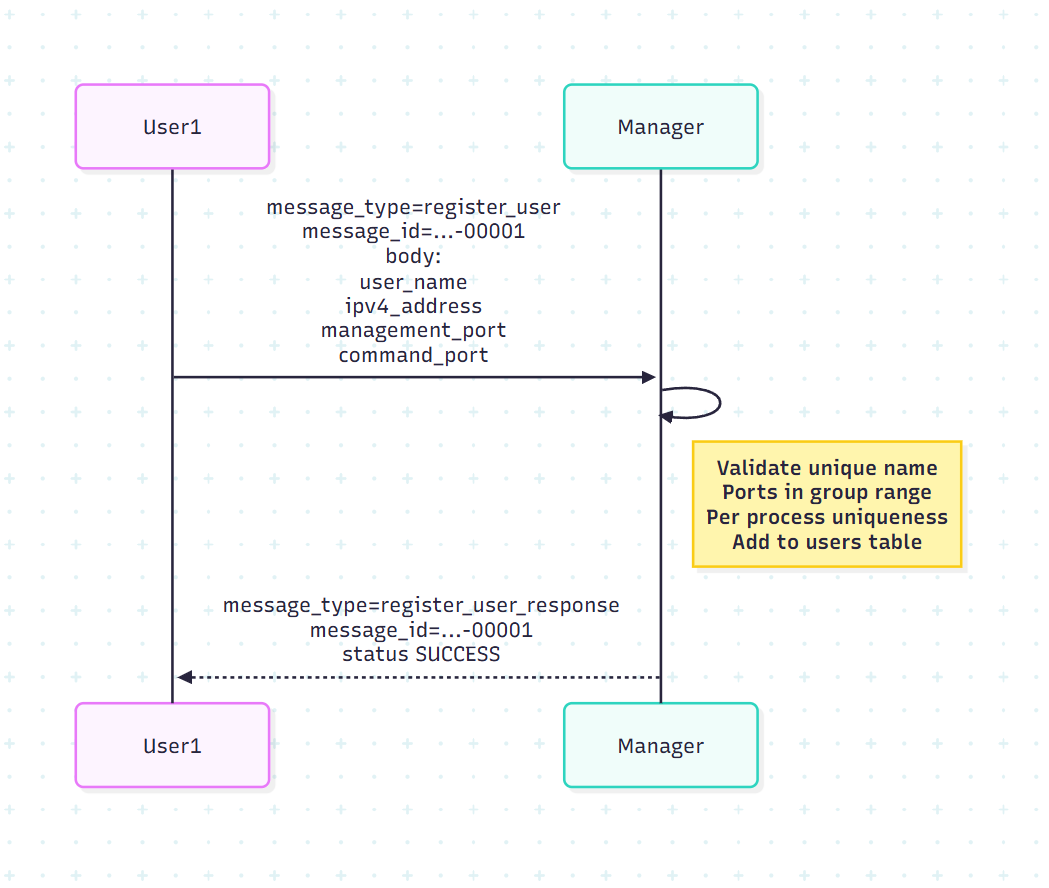
\includegraphics[width=0.95\linewidth]{../screenshots/diagram-screenshots/register-user.png}
  \caption{Time--space diagram for \texttt{register\_user}}
  \label{fig:ts-register-user}
\end{figure}

\subsubsection{Command: \texttt{register\_disk}}
\begin{figure}[H]
  \centering
  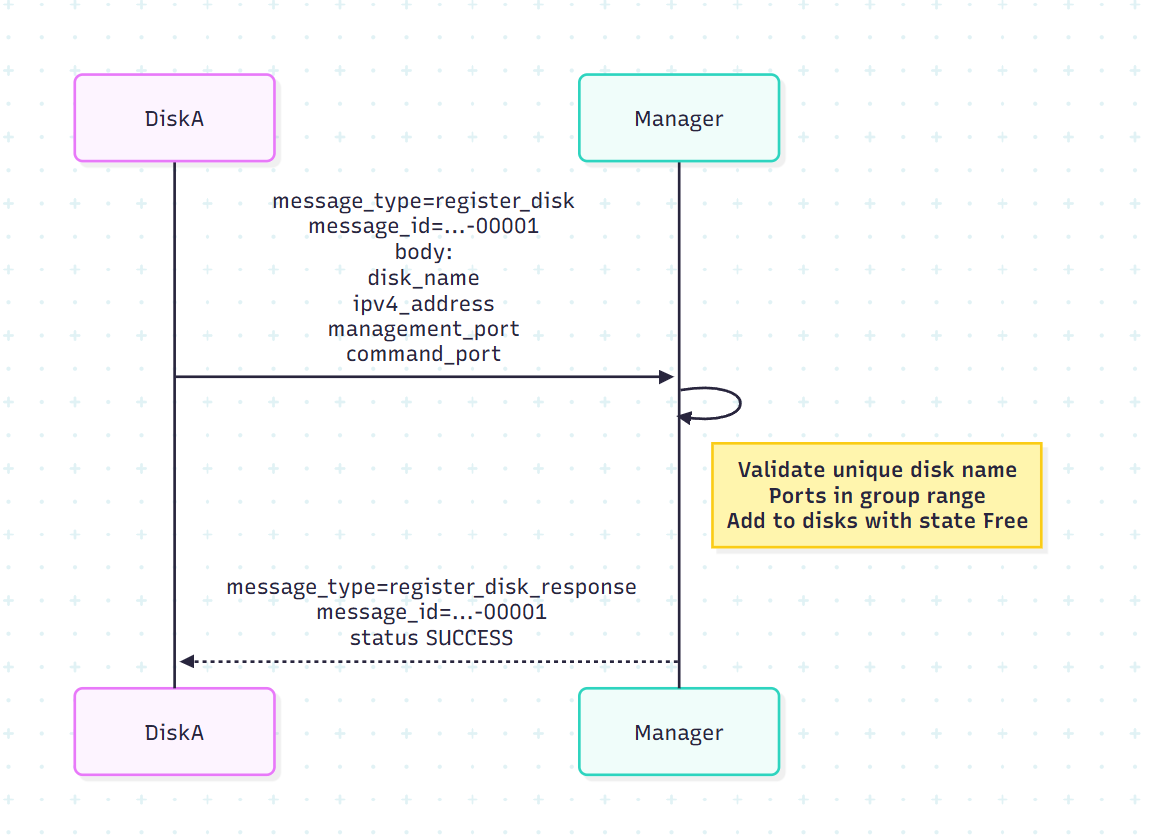
\includegraphics[width=0.95\linewidth]{../screenshots/diagram-screenshots/register-disk.png}
  \caption{Time--space diagram for \texttt{register\_disk}}
  \label{fig:ts-register-disk}
\end{figure}

\subsubsection{Command: \texttt{configure\_dss}}
\begin{figure}[H]
  \centering
  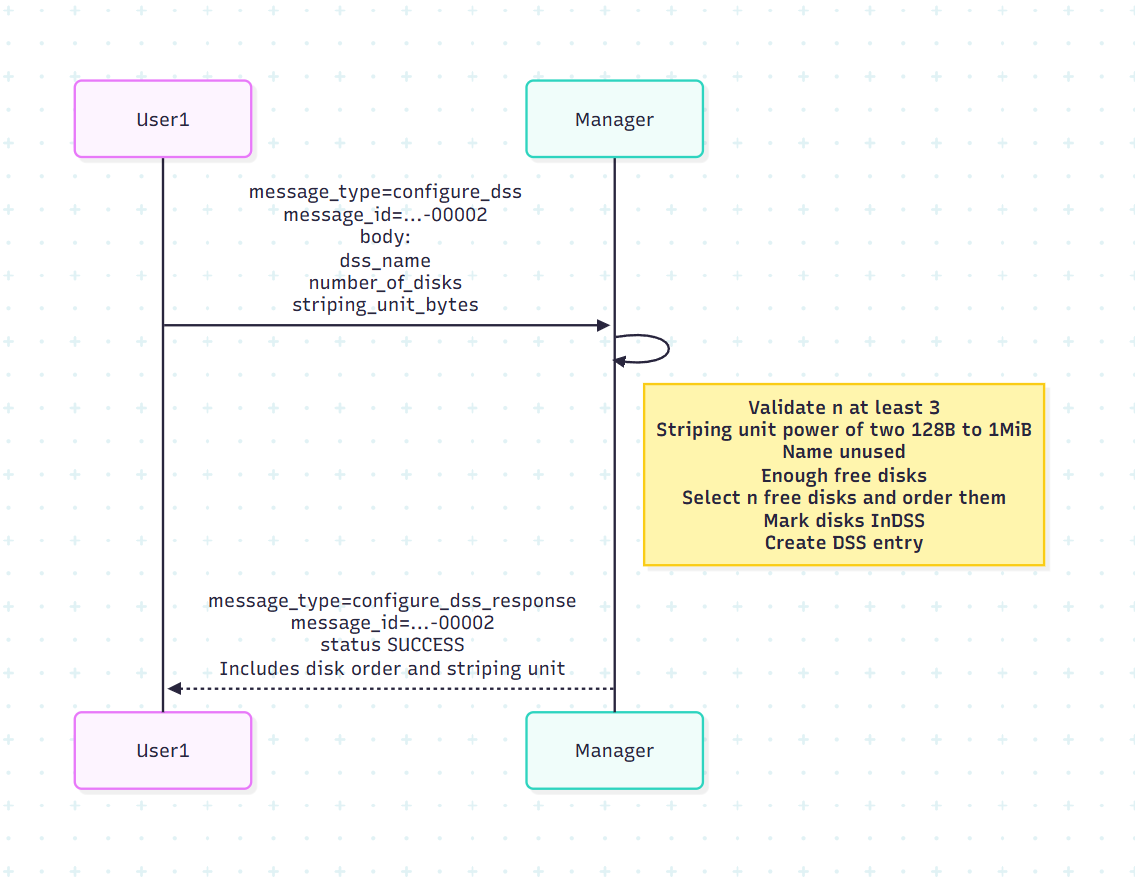
\includegraphics[width=0.95\linewidth]{../screenshots/diagram-screenshots/configure-dss.png}
  \caption{Time--space diagram for \texttt{configure\_dss}}
  \label{fig:ts-configure-dss}
\end{figure}

\subsubsection{Command: \texttt{deregister\_user}}
\begin{figure}[H]
  \centering
  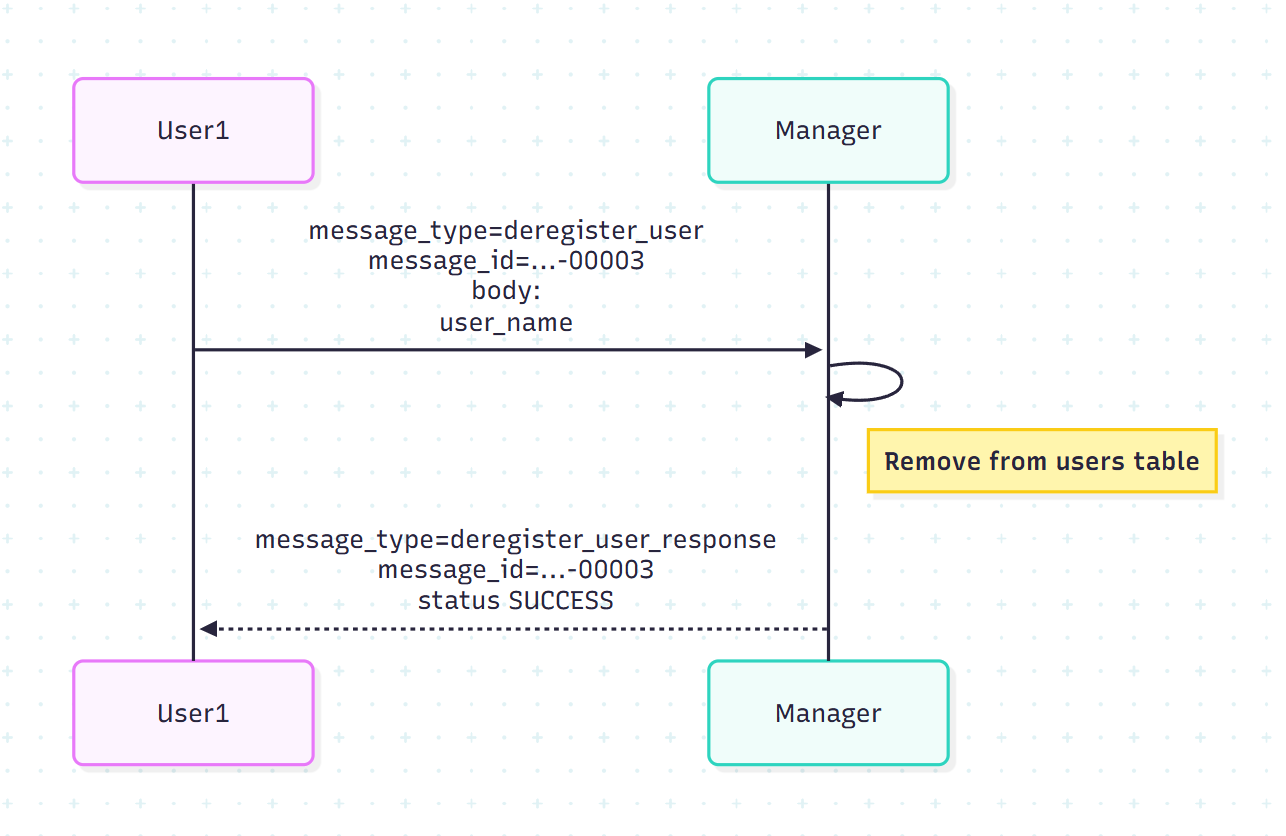
\includegraphics[width=0.95\linewidth]{../screenshots/diagram-screenshots/deregister_user.png}
  \caption{Time--space diagram for \texttt{deregister\_user}}
  \label{fig:ts-deregister-user}
\end{figure}

\subsubsection{Command: \texttt{deregister\_disk}}
\begin{figure}[H]
  \centering
  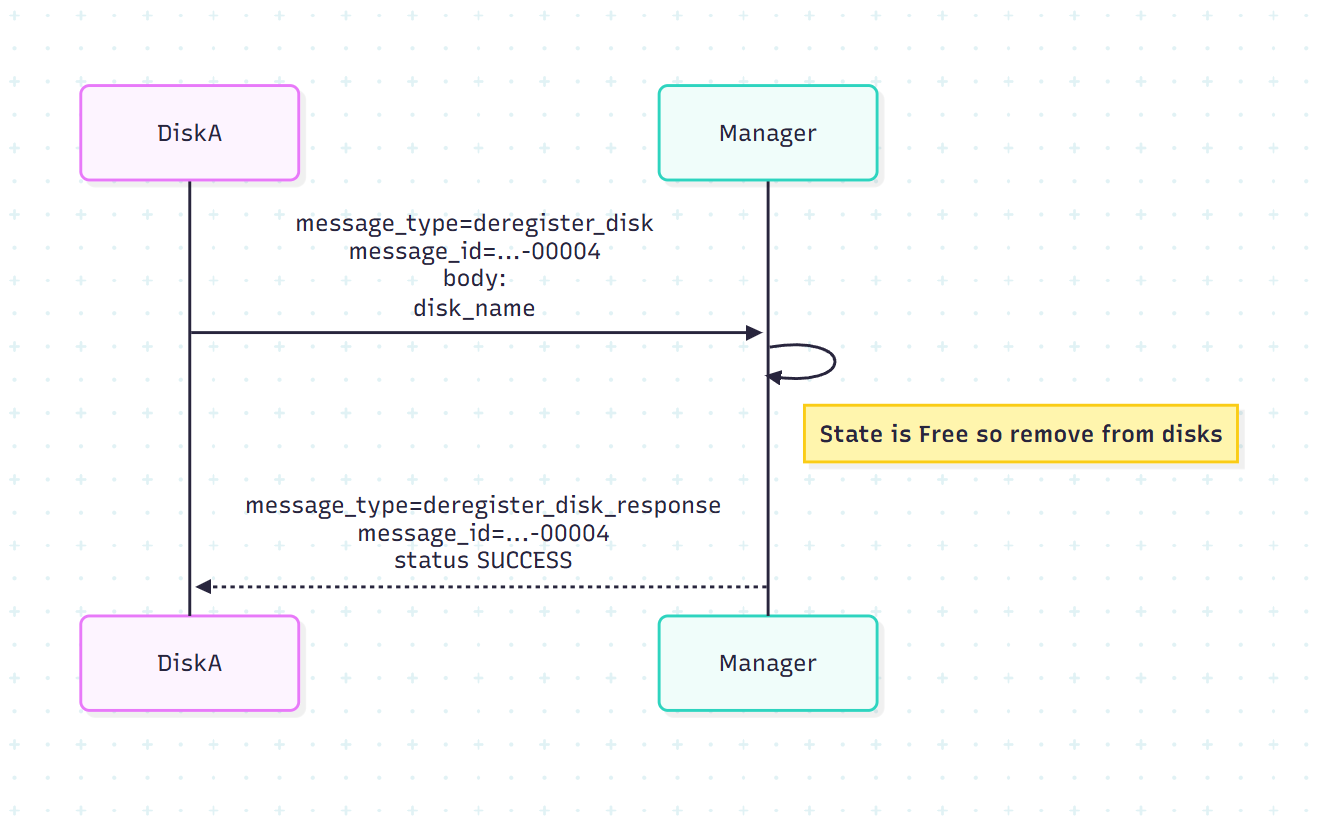
\includegraphics[width=0.95\linewidth]{../screenshots/diagram-screenshots/deregister-disk.png}
  \caption{Time--space diagram for \texttt{deregister\_disk}}
  \label{fig:ts-deregister-disk}
\end{figure}

\subsection{Data Structures and Design Decisions}
\subsubsection{Manager State}
TBD.

\subsubsection{Client/User State}
TBD.

\subsection{Port Numbers}
Because I am Group 198, the port numbers are 21200–21299 (inclusive).

\subsection{Screenshots}
Provide the following screenshots (place files under \texttt{screenshots/}):
\begin{enumerate}[label=\roman*.]
  \item Output of: \texttt{git log --pretty=format:"\%h - \%an, \%ad (Commit) - \%cd (Author)"} \; (TBD)
  \item Entire commit history of the GitHub repository (TBD)
  \item Output of: \texttt{git reflog} (TBD)
  \item Output of: \texttt{git fsck} (TBD)
\end{enumerate}

\begin{figure}[h]
  \centering
  % \includegraphics[width=\linewidth]{screenshots/git-log.png}
  \fbox{\parbox{0.9\linewidth}{TBD: Insert screenshot of git log command output}}
  \caption{\texttt{git log} output}
  \label{fig:git-log}
\end{figure}

\begin{figure}[h]
  \centering
  % \includegraphics[width=\linewidth]{screenshots/commit-history.png}
  \fbox{\parbox{0.9\linewidth}{TBD: Insert screenshot of full commit history}}
  \caption{Repository commit history}
  \label{fig:commit-history}
\end{figure}

\begin{figure}[h]
  \centering
  % \includegraphics[width=\linewidth]{screenshots/git-reflog.png}
  \fbox{\parbox{0.9\linewidth}{TBD: Insert screenshot of \texttt{git reflog} output}}
  \caption{\texttt{git reflog} output}
  \label{fig:git-reflog}
\end{figure}

\begin{figure}[h]
  \centering
  % \includegraphics[width=\linewidth]{screenshots/git-fsck.png}
  \fbox{\parbox{0.9\linewidth}{TBD: Insert screenshot of \texttt{git fsck} output}}
  \caption{\texttt{git fsck} output}
  \label{fig:git-fsck}
\end{figure}

\subsection{Video Demo Link and Timestamps (3(a)--3(f))}
\paragraph{Accessible Link} \url{TBD}
\paragraph{Timestamps} TBD.
\begin{enumerate}
  \item 3(a): TBD
  \item 3(b): TBD
  \item 3(c): TBD
  \item 3(d): TBD
  \item 3(e): TBD
  \item 3(f): TBD
\end{enumerate}

\section{Extended Design for Full Project (30\%)}
\subsection{Additional Commands Implemented}
TBD.

\subsubsection{Command: \texttt{<NAME>}}
\paragraph{Purpose} TBD.
\paragraph{Request Message Format} TBD.
\paragraph{Response Message Format} TBD.
\paragraph{Error Handling} TBD.

\subsection{Updated Design Decisions and Use of Threads}
TBD.

\subsection{Screenshots (Repeat Items from Step 1 of \S4.1)}
TBD.

\subsection{Video Timestamps (3(a)--3(h))}
\begin{enumerate}
  \item 3(a): TBD
  \item 3(b): TBD
  \item 3(c): TBD
  \item 3(d): TBD
  \item 3(e): TBD
  \item 3(f): TBD
  \item 3(g): TBD
  \item 3(h): TBD
\end{enumerate}

\appendix
\section{Message Format Template}
TBD.

\section{Time--Space Diagram Notes}
TBD.

\end{document}
